

\documentclass[../../e1_tp1_main.tex]{subfiles}

\begin{document}
\chapter{Ejercicio 3}

Se construyó el siguiente circuito

\begin{figure}[H]
\centering
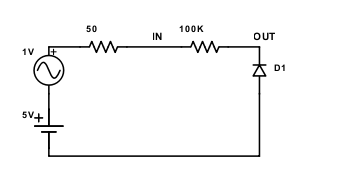
\includegraphics[width=0.5\textwidth]{imagenes/cirq.png}
\caption{Circuito}
\end{figure}


\section{Modelo del diodo en AC}

El dido en corriente alterna (pequeñas amplitudes), se puede modelar como el paralelo de un capacitor con una resistencia. La resitencia es la resistencia dinamica del dido, la cual se mantiene constante devido a la vaja amplitud de alterna. La capacidad del didodo proviene de dos fenomenos distintos, uno de los fenomenos es la capacidad proveniente de la juntura. Devido a que  la juntura se la puede modelar como un dielectrico y a ambos lados de discho dielectrico hay cargas, por ende se obtiene un capacitor de placas paralelas. El segundo fenomeno es la capacidad de difusión.

\begin{figure}[H]
\centering
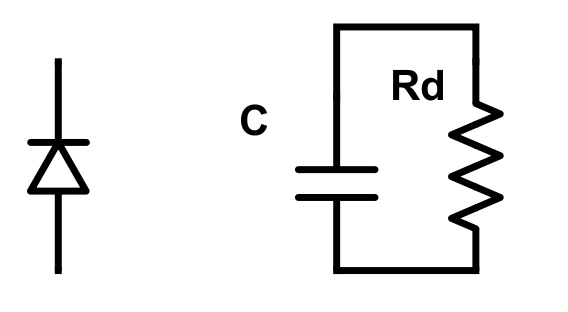
\includegraphics[width=0.5\textwidth]{imagenes/modAc.png}
\caption{Modelo ac del diodo}
\end{figure}

\section{Funcion transferencia}

Teniendo en cuenta el modelo del diodo, y aplicando divisor de tensión, se obtiene la funscion transferencia del circuito.

\begin{equation}
H(S)=\frac{R_D}{R + R_D} \frac{1}{1+ \frac{S}{\frac{R+R_D}{C R_d}}}
\end{equation}

La funcion transferencia hallada, corresponde a un sistema de orden 1, sus la parte real de su polo es negativa, por ende el sistema es BIBO estable. Para hallar la respuesta en frecuencia, basta evaluar $S=jW$. El sistema posee la forma de un pasa bajos $H(S)=\frac{K}{1+\frac{S}{W_C}}$,  por ende se esperaria que una decada antes de la frecuencia de corte $W_C$ no deveria haber atenuacion, en la frecuencia de corte deveria atenuar 3dB, y posterior a la frecuencia de corte se esperarian una tenuacion de 20dB por decada (sistema de primer orden). En cuanto a la fase, se esperaria que varie entre 0  y -90 pasando por -45 en la frecuencia de corte.
\\
De la hoja de datos del 1N4007 obtuvimos que su capacitancia es de aproximadamente 8 pF.

\begin{figure}[H]
\centering
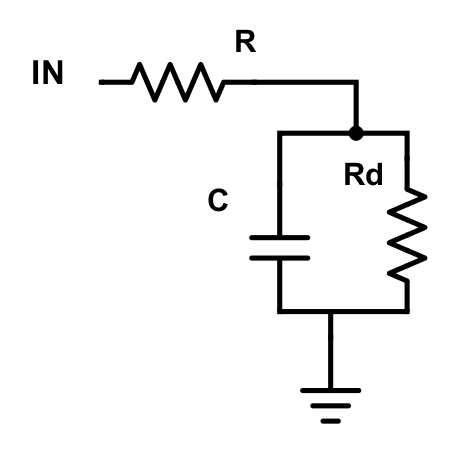
\includegraphics[width=0.45\textwidth]{imagenes/modCD.png}
\caption{circuito con modelo ac del diodo}
\end{figure}
\section{Mediciones}

Las mediciones se realizaron con un generador de funciones y un osiloscoppio. Las puntas del osiloscopio se configuraron en por 1.

\begin{figure}[H]
\centering
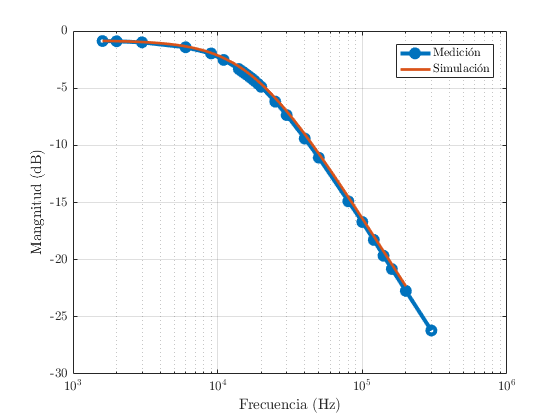
\includegraphics[width=0.75\textwidth]{imagenes/mag.png}
\caption{magnitud medida y simulada}
\end{figure}

\begin{figure}[H]
\centering
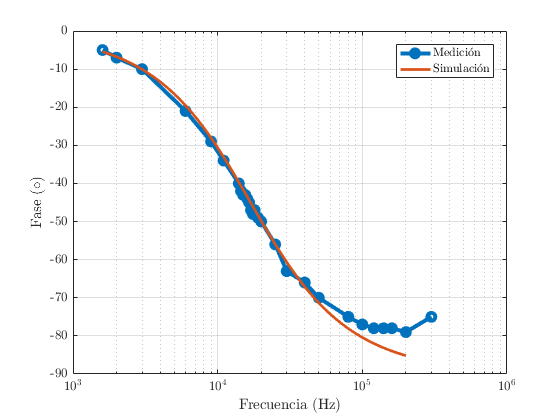
\includegraphics[width=0.75\textwidth]{imagenes/fase.png}
\caption{fase medida y simulada}
\end{figure}

\section{Conclusión}

Como se observan en los graficos de las mediciones la simulacion ajusta a lo meido. Sin embargo, para que esto suceda en la simulacion se tuvo en cuanta los efectos de las puntas del osiloscopio, modeladas como el paralelo de un capacitor de 100pF con una resistencia de $1M \Omega $, alterando el comportamiento predicho. Ademas $R_D$, no se puede considerar constante, devido a que el circuito se alimento con una tencion 1 v peak-to-peak, lo cual no se considera una señal pequeña.

\end{document}

